\chapter{\iflanguage{ngerman}{Technischer Hintergrund}{Background}}
\label{sec:background}

%%%%%%%%%%%%%%%%%%%%%
%       ROS2        %
%%%%%%%%%%%%%%%%%%%%%
\section{\gls{ros2}}
The \gls{ros} is not an operating system in the classical sense. Rather, ROS can be understood as a lightweight open-source collection of various software packages for robot development. It is a middleware that brings hardware abstraction, package management and communication between processes \cite{quigley_ros_nodate, noauthor_ros_nodate}.\newline
\gls{ros} however, has its limitations regarding security, reliability in non-traditional environments, and support for large scale embedded systems. \gls{ros2} is the second redesigned generation of \gls{ros}. \gls{ros2} was developed from the ground up with the goal of overcoming these challenges \cite{rico_concise_2022, macenski_robot_2022, liao_introduction_2020}.
\begin{figure}[htbp]
	\centering
	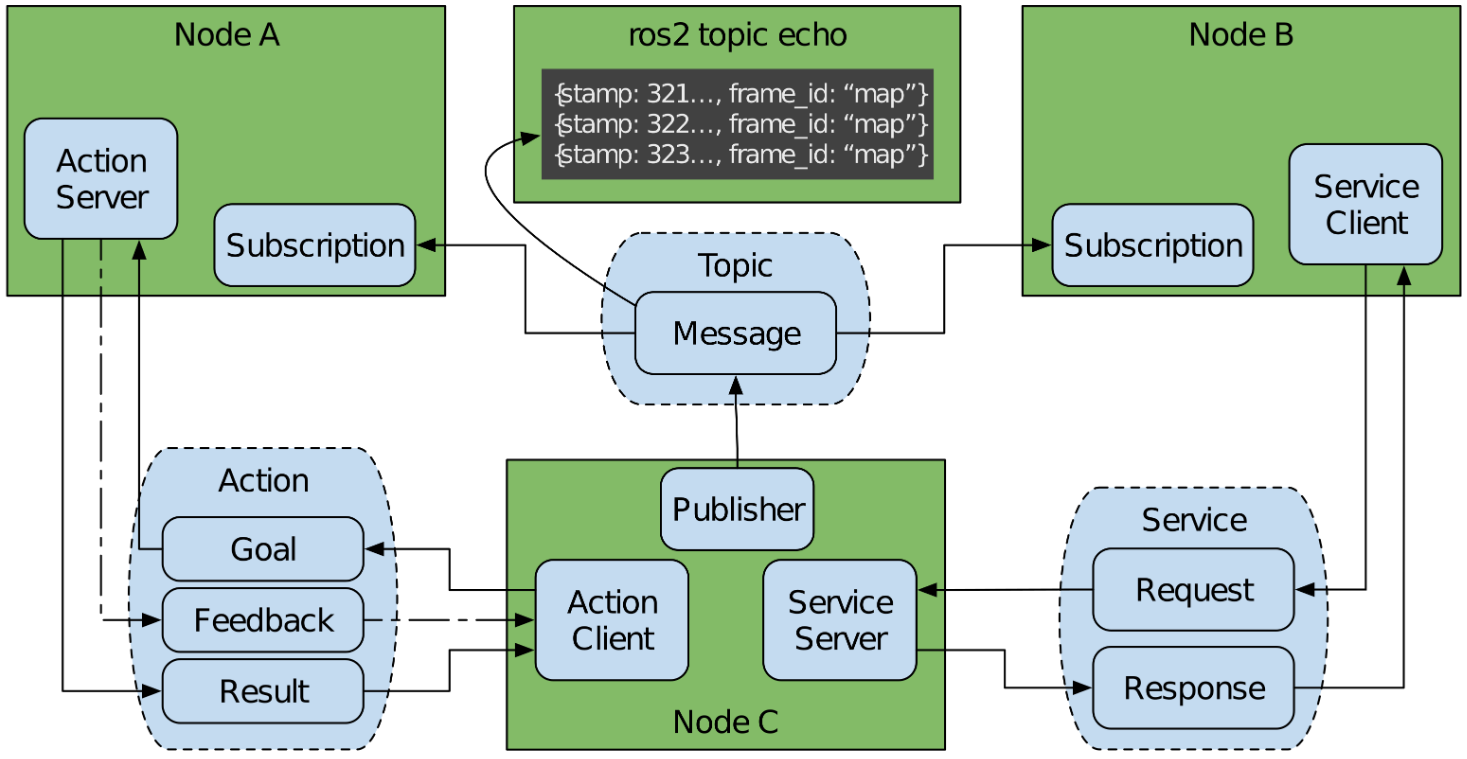
\includegraphics[width=1\textwidth]{Figures/c3/ros2_node_interfaces.png}
	\caption{Different communication patterns in \gls{ros2} organized under the \gls{node} interface \cite{macenski_robot_2022}.}
	\label{c3_fig_ros2_node_interfaces}
\end{figure}
It is an open source software development kit distributed under the Apache 2.0 License and can be split into three categories. The middleware, algorithms and developer tools \cite{macenski_robot_2022}. 
Written software can be divided thereby in dedicated parts, so-called \glspl{node}. In \gls{ros2} there is unified API which allows creating multiple communication patterns under the concept of \glspl{node}. This is represented in figure \ref{c3_fig_ros2_node_interfaces}. The most important concepts for this thesis are: \glspl{topic} and \glspl{service}. \Glspl{topic} provide an interface for passing \glspl{message} in an asynchronous manner. \Glspl{service} on the other hand, allow exchange of data in a request-response style pattern. Here, it is not mandatory that the client making the request blocks until the response arrives \cite{rico_concise_2022, macenski_robot_2022}.\newline
In figure \ref{c3_fig_ros2_stack} the client library API stack of \gls{ros2} is shown. \gls{ros2} follows earlier design philosophies and consists of several abstraction layers distributed across different packages. These layers allow multiple solutions for needed functions and allow users to replace components or select specific parts of the system that they need. Most users interact with the client libraries like \gls{rclcpp} and \gls{rclpy}. The \gls{rclcpp} and \gls{rclpy} libraries provide access to the main communication APIs and are tailored to specific programming languages. \gls{ros2} supports distributed computing on multiple machines and processes, including integration with cloud resources. It uses an intermediate interface called \gls{rcl} for common functions, and underneath, the middleware abstraction layer called \gls{rmw} provides key communication interfaces. Different \gls{rmw} implementations representing different middleware technologies can be used interchangeably depending on performance, licensing, or platform requirements \cite{rico_concise_2022, macenski_robot_2022, liao_introduction_2020}. \newline
The \gls{rmw} should be agnostic to \gls{dds} and the default middleware used in \gls{ros2} is eProsima's FastDDS \cite{macenski_robot_2022, noauthor_ros_nodate-1, noauthor_eprosima_nodate}. A more detailed introduction to \gls{dds} and to different implementations of \gls{dds} is given in section \ref{c3_sec_dds}.
\begin{figure}[htbp]
	\centering
	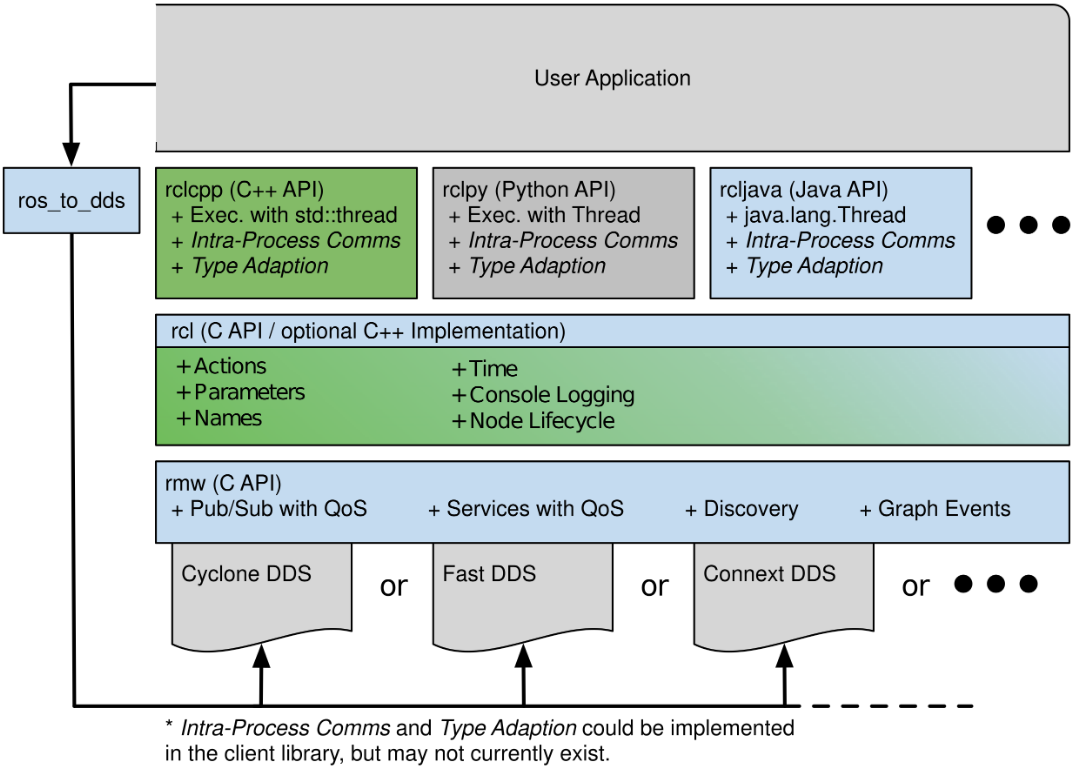
\includegraphics[width=1\textwidth]{Figures/c3/ros2_client_library_stack.png}
	\caption{The \gls{ros2} client library API stack with the support of different \gls{dds} implementations shown \cite{macenski_robot_2022}.}
	\label{c3_fig_ros2_stack}
\end{figure}

%%%%%%%%%%%%%%%%%%%%%%%%%%%%%%%%%%%%%%%%%%%%%%%%%
%   Data Exchange in Real-Time over Networks    %
%%%%%%%%%%%%%%%%%%%%%%%%%%%%%%%%%%%%%%%%%%%%%%%%%
\section{OMG Data Distribution Service}\label{c3_sec_dds}
The \glsentryfull{dds} is an open international middleware standard for real-time and embedded systems\cite{noauthor_data_nodate}. It is designed to facilitate efficient and reliable communication between distributed systems and devices in a wide range of industries.\newline 
\gls{dds} provides a data-centric publish-subscribe communication model, where data producers (publishers) publish data on specific topics, and data consumers (subscribers) can subscribe to those topics. The subscriber then receives the corresponding data via the topic. \gls{dds} ensures that the data is delivered reliably and in a timely manner to all interested subscribers. \cite{pardo-castellote_omg_2003, schlesselman_omg_2004}.

Some of the key features of \gls{dds} are listed below:\todo{rewrite!!!!}
\begin{itemize}
    \item \gls{qos}: \gls{dds} allows fine-grained control over various quality-of-service parameters to meet the specific requirements of different applications. \gls{qos} settings include reliability, bandwidth, delivery deadlines, and resource limits.

    \item Data-centricity: \gls{dds} focuses on the data itself, rather than the underlying transport or network infrastructure. It enables decoupling of data producers and consumers, allowing flexible and dynamic system configurations.

    \item Scalability: \gls{dds} supports both local and distributed systems, allowing seamless communication across multiple nodes, networks, or even geographically dispersed systems. It can handle large-scale deployments with high data rates and low latency.

    \item Interoperability: \gls{dds} promotes interoperability between different vendors and platforms. Applications built using \gls{dds} can communicate with each other regardless of the programming language, operating system, or hardware used, as long as they adhere to the \gls{dds} standard.

    \item Extensibility: \gls{dds} provides a modular and extensible architecture, allowing additional functionality and customizations to be added through optional extensions and profiles.

\end{itemize}
\subsection{DDS Vendors and Implementations}
For \gls{dds} exist a variety of different vendors and implementations. In table \ref{c3_tab_overview_rmw} an overview of a few different \gls{dds} implementations used as \gls{rmw} is given.
\subsubsection*{Fast \gls{dds}}
Fast \gls{dds} by eProsima is the default \gls{rmw} used since \gls{ros2} Foxy. It is at the time of writing still used as the default \gls{rmw} for \gls{ros2} Rolling. As the default \gls{rmw} it is fully supported and deployed under an Apache 2 license together with the binary releases. \cite{noauthor_dds_nodate-1} 
\subsubsection*{Cyclone \gls{dds}}
Eclipse Cyclone \gls{dds}\textsuperscript{\texttrademark} is an implementation of the OMG \gls{dds} together with an implementation of the \gls{dds} Interoperability Wire Protocol (DDSI-RTPS\textsuperscript{\texttrademark}). It is a tier-1 \gls{rmw} and therefore fully supported. On Kubuntu it can either be installed via Debian packages as binary or from source. The middleware implementation is completely open source and distributed under Eclipse Distribution License 1.0 (BSD) and Eclipse Public License 2.0. \cite{anonymous_eclipse_2017, noauthor_eclipse_nodate}
\subsubsection*{Connext \gls{dds}}
Connext \gls{dds} is an implementation by RTI. It is fully supported as well, but only a binary installation via Debian packages is available. It is either commercially or for research purpose available. \cite{innovations_connext_nodate, noauthor_documentation_nodate}
% \subsubsection*{Zenoh}\todo{Write}
% Zenoh is a publisher, subscriber and query protocol by the Eclipse foundation.
% \href{https://www.adlinktech.com/en/Zenoh}{Zenoh} 
% \href{https://zenoh.io/blog/2021-03-23-discovery/}{Zenoh advantages} 

\begin{table}[htbp]
    \centering
\begin{tabular}{ |c|c|c|c| }
\hline
\multicolumn{4}{|c|}{Overview of the used \gls{rmw}s} \\
\hline
Product name & License & \gls{rmw} implementation & status  \\
\hline
\hline
eProsima Fast \gls{dds} & Apache 2 & rmw\_fastrtps\_cpp & 
    \begin{minipage}{4.2cm}
	    \vskip 8pt
		  Full support. \textbf{Default} \textbf{RMW}. Packaged with binary releases.
	    \vskip 8pt
	\end{minipage} \\\hline
 Eclipse Cyclone \gls{dds} & \begin{minipage}{2cm} \vskip 8pt Eclipse Public License v2.0 \vskip 8pt\end{minipage} & rmw\_cyclone\gls{dds}\_cpp & 
    \begin{minipage}{4.2cm}
	   \vskip 8pt
      Full support. Packaged with binary releases.\newline\newline
	   \vskip 8pt
	\end{minipage} \\\hline
 RTI Connext \gls{dds} & \begin{minipage}{2cm} \vskip 8pt commercial, research \vskip 8pt\end{minipage} & rmw\_connext\_cpp & 
    \begin{minipage}{4.2cm}
	   \vskip 8pt
		 Full support. Support included in binaries, but Connext installed separately.
	   \vskip 8pt
	\end{minipage} \\\hline%\hline
 %  Eclipse Zenoh & Apache 2 & $-$ & \begin{minipage}{4.2cm}
	%  \vskip 8pt
	% 	 Via Zenoh bridge for \gls{dds}. \gls{dds} publisher/subscribers are mirrored and communication routed through Zenoh.
	%  \vskip 8pt
	% \end{minipage} \\\hline
\end{tabular}
    \caption{Overview of the different \glspl{rmw} used for comparison.}\label{c3_tab_overview_rmw} %Eclipse Zenoh is not a \gls{rmw} implementation, but there exists a plugin, called \texttt{zenoh-plugin-\gls{dds}}, which allows to route the \gls{dds} traffic through Zenoh.}
\end{table}

\section{Real-Time Capability of \gls{ros2}}
For a result to be valid in a real-time system, not only must the result be correct, but the time at which the result was generated is also important. Real-time systems can be divided into soft, firm and hard real-time. In a soft real-time system, the deadline can be exceeded within certain limits without causing fatal system conditions. In both fixed and hard real-time systems, the deadline must not be exceeded. The difference is that in firm real-time systems the current execution is aborted without fatal system conditions if the deadline is exceeded. In hard real-time systems, however, exceeding the deadline leads to fatal system conditions.\newline
As already described in section described in section \ref{c2_sec_control_over_network} Gutiérrez et al. conducted some experiments regarding the capabilities of \gls{ros2} to provide real-time communication. They concluded soft real-time to be possible, but not hard \cite{gutierrez_towards_2018}. In further investigations, Puck et al. even suggested hard real-time to be possible with the correct system configuration \cite{puck_performance_2021}. One important factor is the real-time capably of the underlying operating system and the used network stack.

\subsection{Preempt-RT}
Linux distributions like Ubuntu, are not real-time capable out of the box. Preempt-RT is a patch for the Linux kernel, commonly used to enhance the Linux kernel with real-time capabilities \cite{noauthor_realtimestart_nodate}. The kernel patch does not provide hard real-time, since those require a proof that the given deadlines are met. For a complex operating system like Ubuntu such proofs become unfeasible \cite{puck_distributed_2020}. However, the patch provides soft real-time capabilities by allowing preemption anywhere in the Linux kernel and additional features to improve scheduling determinism.

%%%%%%%%%%%%%%%%%%%%%%%%%%%%%%%%%
%   The ros2_control Framework  %
%%%%%%%%%%%%%%%%%%%%%%%%%%%%%%%%%
\section{The \gls{r2c} Framework}\label{ros2_control}
The open-source framework \gls{r2c}, is a framework for real-time control, initially released for \gls{ros2} Foxy. It is a rewrite of \gls{rc}, with the goal to simplify integration of new hardware and overcome some drawbacks present in \gls{rc} \cite{noauthor_welcome_nodate, magyar_getting_started_with_ros2_control_2021, magyar_ros2_control_the_future_of_ros_control_2021}. As shown in table \ref{c3_tab_r2c_repos} the framework comprises multiple repositories. It includes core functionality like management of controllers and hardware, as well as implementations of commonly used controllers. Besides, it provides low-level tools for control theory and real-time control. \newline
A more detailed view of the internals of the \gls{r2c} framework is presented in figure \ref{c3_fig_ros2_control_uml}. As can be seen, the framework includes a controller manager. The controller 
\begin{table}[htbp]
    \centering
\begin{tabular}{ |c|c| }
\hline
\multicolumn{2}{|c|}{\gls{r2c} repositories} \\
\hline
Repository & Description  \\
\hline
\hline
\href{https://github.com/ros-controls/ros2_control}{ros2\_control} 
 & \begin{minipage}{11cm}
	 \vskip 8pt
		 Core functionality like controller manager, resource manager, interfaces for hardware abstraction, and more.
	 \vskip 8pt
	\end{minipage}  \\
\href{https://github.com/ros-controls/ros2_controllers}{ros2\_controllers}  & \begin{minipage}{11cm}
	 \vskip 8pt
		 Collection of commonly and widely used controllers like forward command controller, joint trajectory, \dots
	 \vskip 8pt
	\end{minipage}  \\
\href{https://github.com/ros-controls/control_toolbox}{control\_toolbox}  & \begin{minipage}{11cm}
	 \vskip 8pt
		Control theory implementations (e.g. PID) used by controllers.
	 \vskip 8pt
	\end{minipage}  \\
\href{https://github.com/ros-controls/realtime_tools}{realtime\_tools}  & \begin{minipage}{11cm}
	 \vskip 8pt
		 Toolkit for real-time use. It includes e.g. real-time buffers and real-time publishers.
	 \vskip 8pt
	\end{minipage}  \\
\href{https://github.com/ros-controls/control_msgs}{control\_msgs}   & \begin{minipage}{11cm}
	 \vskip 8pt
		 Common messages used within the framework.
	 \vskip 8pt
	\end{minipage}  \\
\hline
\end{tabular}
    \caption{Overview of the repositories the \gls{r2c} framework includes.}
    \label{c3_tab_r2c_repos}
\end{table}
manager serves as entry-point for users and provides \gls{ros2} services through which the user can interact with the system. Additionally, it is responsible for managing the controllers and connects them to the abstracted hardware. The abstraction from the physical hardware and drivers is handled by the resource manager. The resource manager is part of the controller manager. Moreover, the resource manager stores and manages the hardware inside a resource storage. The hardware abstraction is done through interfaces (called \textit{hardware components}). These \textit{hardware components} can be divided into three groups:
\begin{itemize}
    \item Actuator (\texttt{ActuatorInterface}): Robotic hardware like motors, valves, and other simple 1-\gls{dof} actuators.
    \item Sensor (\texttt{SensorInterface}): Robotic hardware that can sens and measure physical properties of the environment.
    \item System (\texttt{SystemInterface}): Complex multi-\gls{dof} robotic hardware like an industrial robot.
\end{itemize}
 Finally, there is a collection of controllers inside the \texttt{ros2\_controllers} repositories. Controllers are the units responsible fore calculating a system's input. The input is thereby calculated based on the measured error between a reference value and the system's output.\newline
 In conclusion, the framework can roughly be divided into two parts. The first part includes the controllers and the second part embraces the hardware. The controller manager connects those parts and serves as an entry-point for users to interact with the system.

\subsection{The Link between Controllers and Hardware}\label{c3_sec_link_ctrl_hw}
A very important concept to understand for this thesis are the \gls{ci} and the \gls{si}, which are often called \glspl{handle}. As shown in figure \ref{c3_fig_ros2_control_uml} in the middle above, the \gls{ci} and \gls{si} are located between the hardware site and the controller site of the \gls{r2c} framework. They abstract away from the hardware. The hardware then creates the \glspl{handle} and exports them. The resource manager imports the exported \glspl{ci} and \glspl{si}. They are then stored inside the resource storage and the resource manager manages them. \gls{si} grands access to the state of the component, while \gls{ci} additionally enables to write commands to a hardware component. If a controller wants to get access to the hardware, the resource manager creates so-called loans (\textit{LoanedCommandInterface} or \textit{LoanedStateInterface}). Those loaned interfaces are then passed to the controller. The controller can then read the state and write commands to the hardware via those loans.\newline
This whole concept is based on a \gls{sm} architecture. The drivers of the hardware allocate memory where the values of the \gls{ci} and \gls{si} are stored. A pointer to the allocated memory is then passed to the control site of the framework via the \gls{ci} and \gls{si}. 
\begin{figure}[htbp]
	\centering
	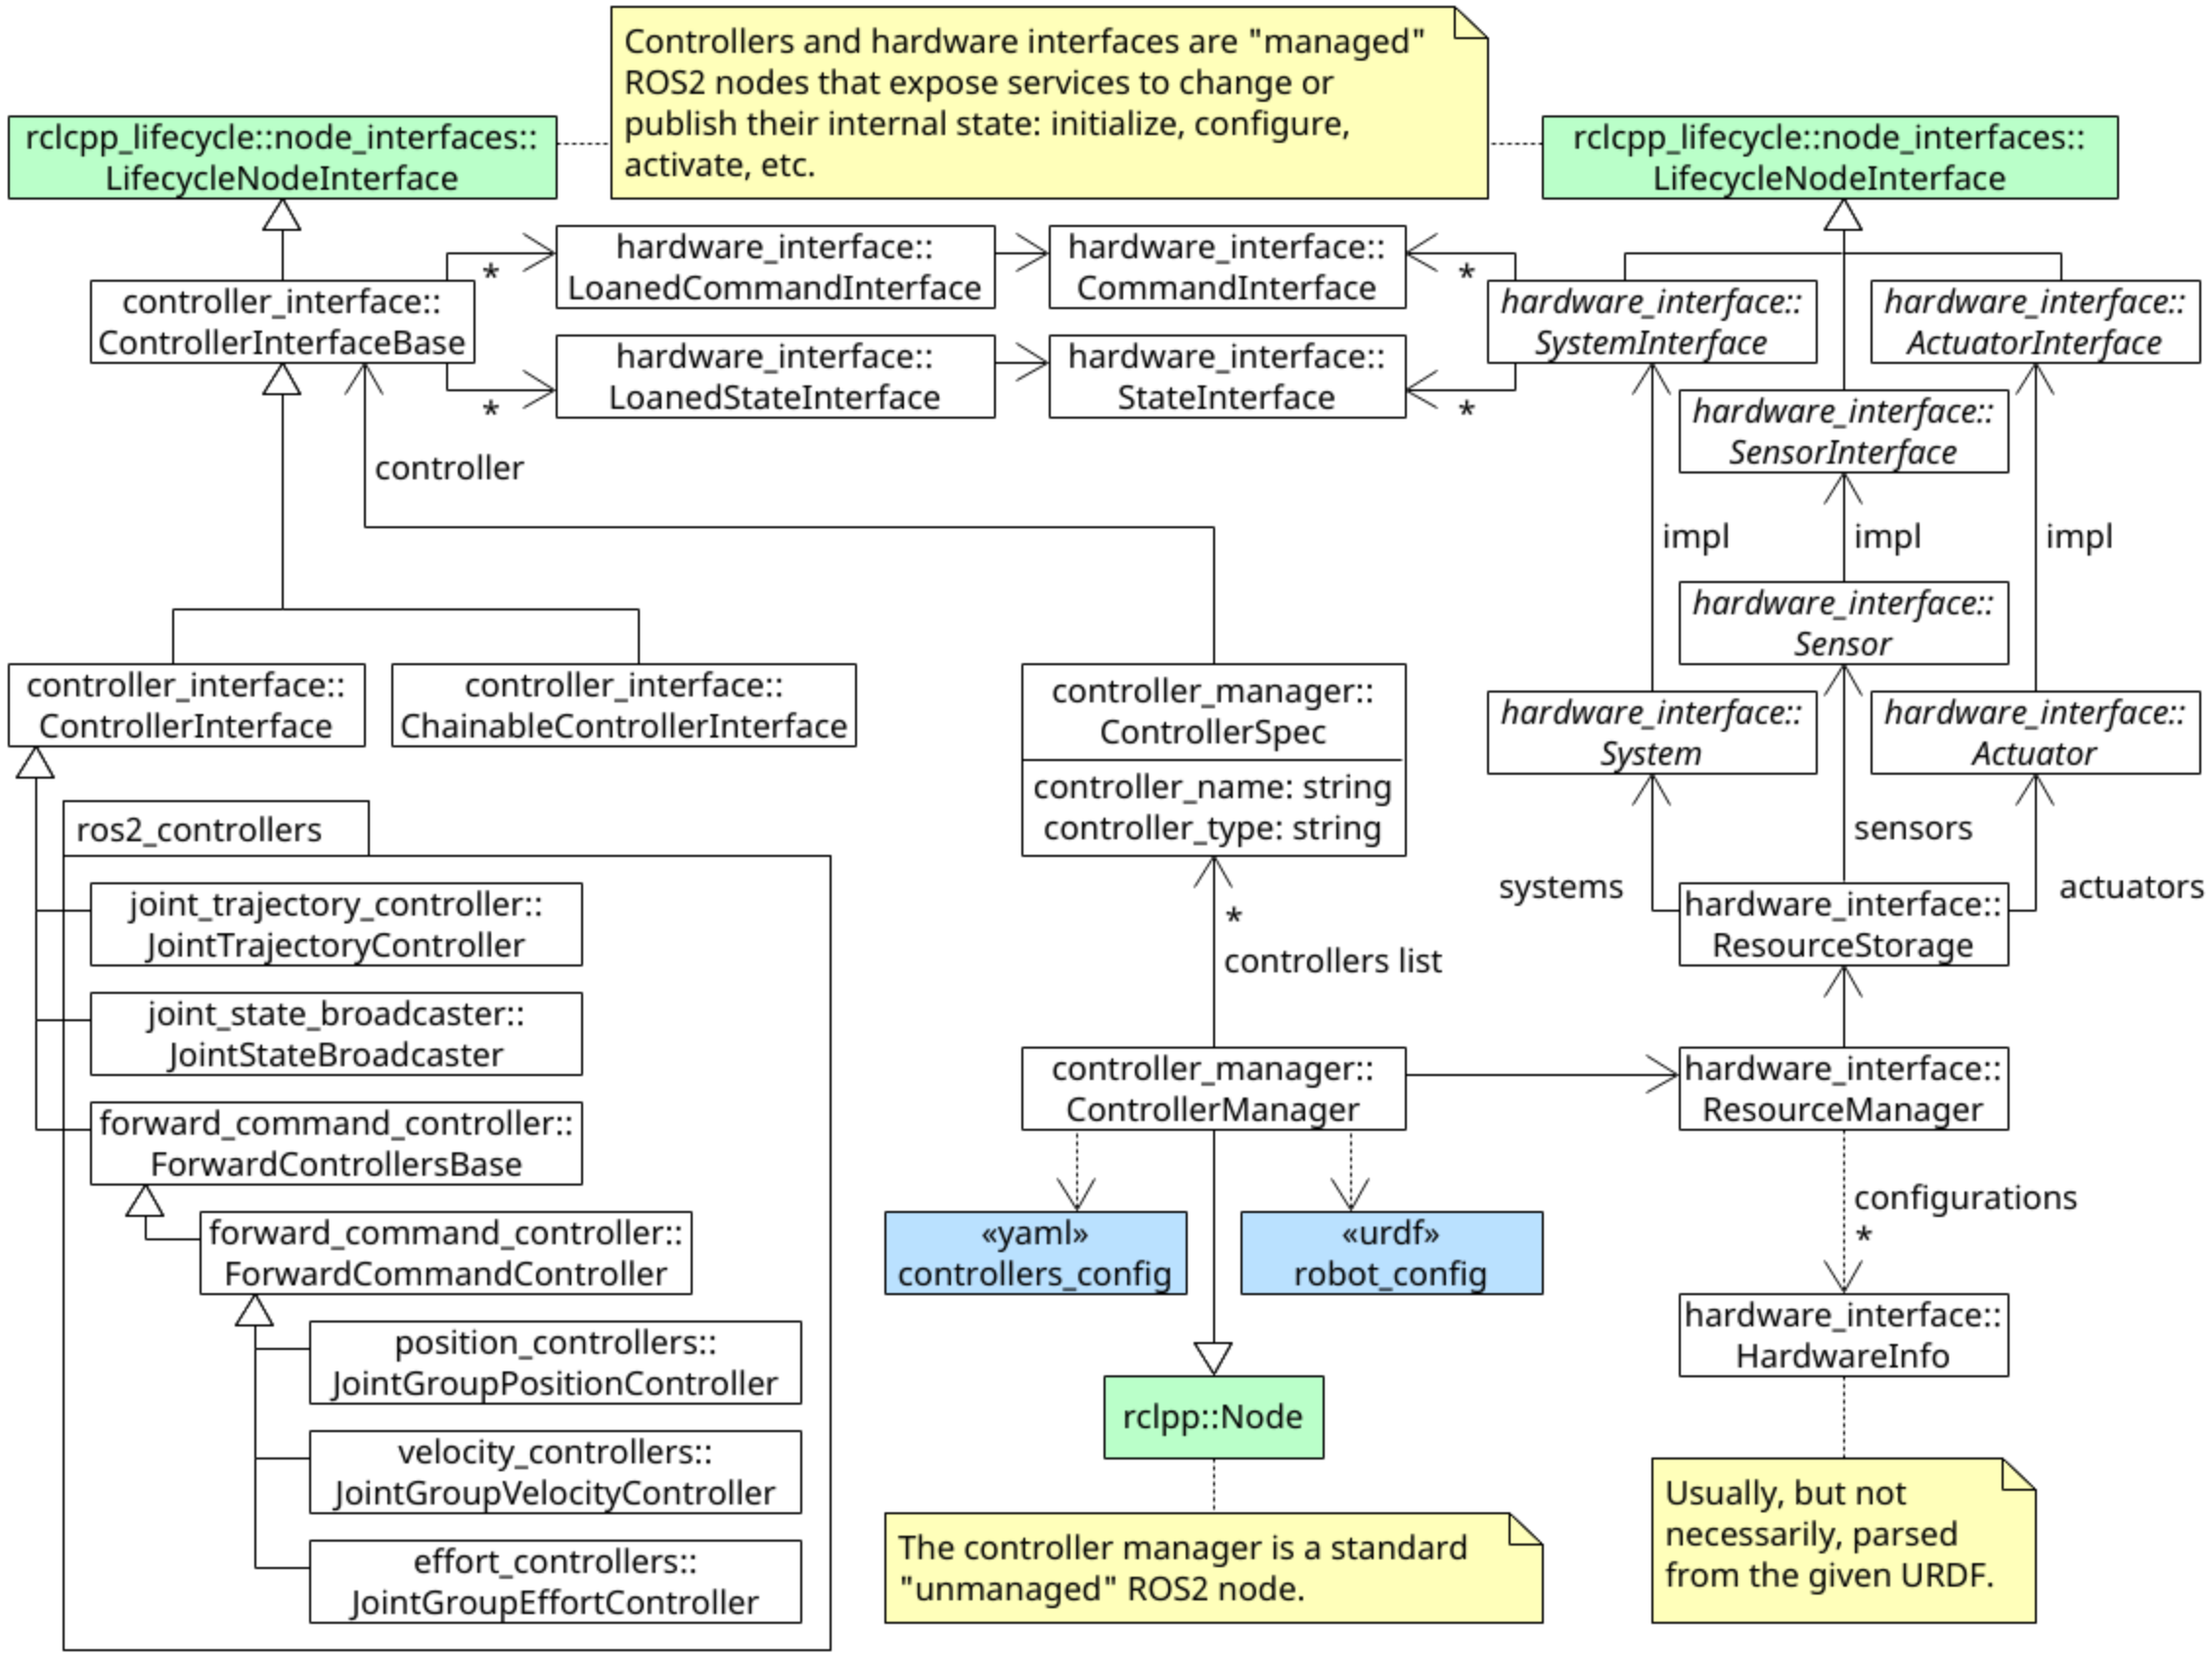
\includegraphics[width=1\textwidth]{Figures/c3/ros2_control_uml.png}
	\caption{UML diagram of the most important classes and interfaces in the \gls{r2c} framework. The \glspl{ci} and \glspl{ci}, so called \glspl{handle}, are of special significance for this thesis. Picture taken from \cite{noauthor_welcome_nodate}. }
	\label{c3_fig_ros2_control_uml}
\end{figure}
 
\subsection{Controller Chaining}
Controller chaining in \gls{r2c} describes the possibility to link the output of one controller to the input of another. The chaining can thereby be in sequence (cascade control) or in parallel.\newline
For a controller to be able to be chained, it has to derive from the \textit{\seqsplit{ChainableController-Interface}} instead of the \textit{ControllerInterface}. The chainable controller must then export reference interfaces. Those reference interfaces have the same meaning as the \glspl{ci}. The controller can then run in either chained or external mode, where the latter is equivalent to a non chainable controller. If the controller runs in chained mode, all external interfaces like subscriber and services are disabled. This is done in order to avoid concurrency in the input commands. Another controller can then claim the reference interfaces and chain its output to the input of the chainable controller.

\subsection{Controlling Multiple Robots with \gls{r2c}}\label{c3_sec_controlling_multiple_robots}
In the current state, \gls{r2c} focuses on controlling a single robot or robot cell. Further, the focus thereby lies on using a single computer to run the whole control stack. This includes the drivers used for communication with the hardware, the controller manager and controllers.\newline
Controlling multiple robots is however possible. Depending on the task, control of multiple robots in the current state of \gls{r2c} can roughly be split into two scenarios.
\begin{enumerate}[start=1,label={\upshape \texttt{Scenario \arabic*:}}, wide = 0pt, leftmargin = 3em]
    \item Task where tight synchronization is needed. $\implies$ One platform with one controller manager. Represented in figure \ref{c3_fig_r2c_mr_ts}.
    \item Task where robots act more or less independent of one another. $\implies$ Multiple platforms with multiple independent controller managers. This can be seen in graphic \ref{c3_fig_r2c_mr_is}.
\end{enumerate}

\paragraph{Scenario 1:} 
In the first scenario, where a tight synchronization between the robots is needed, the most feasible way is to create on controller manager and multiple systems. One system for each robot. Each system can then be controlled by its own controller architecture. The controllers of those architectures are in turn managed by on controller manager. This controller manager can then handle the synchronization between the different systems.\newline
One should note, that this approach is limited to one machine. In the current form of \gls{r2c} there is no way to communicate between multiple controller managers. An outline of the architecture is given in representation \ref{c3_fig_r2c_mr_ts}.
\begin{figure}[htbp]
	\centering
	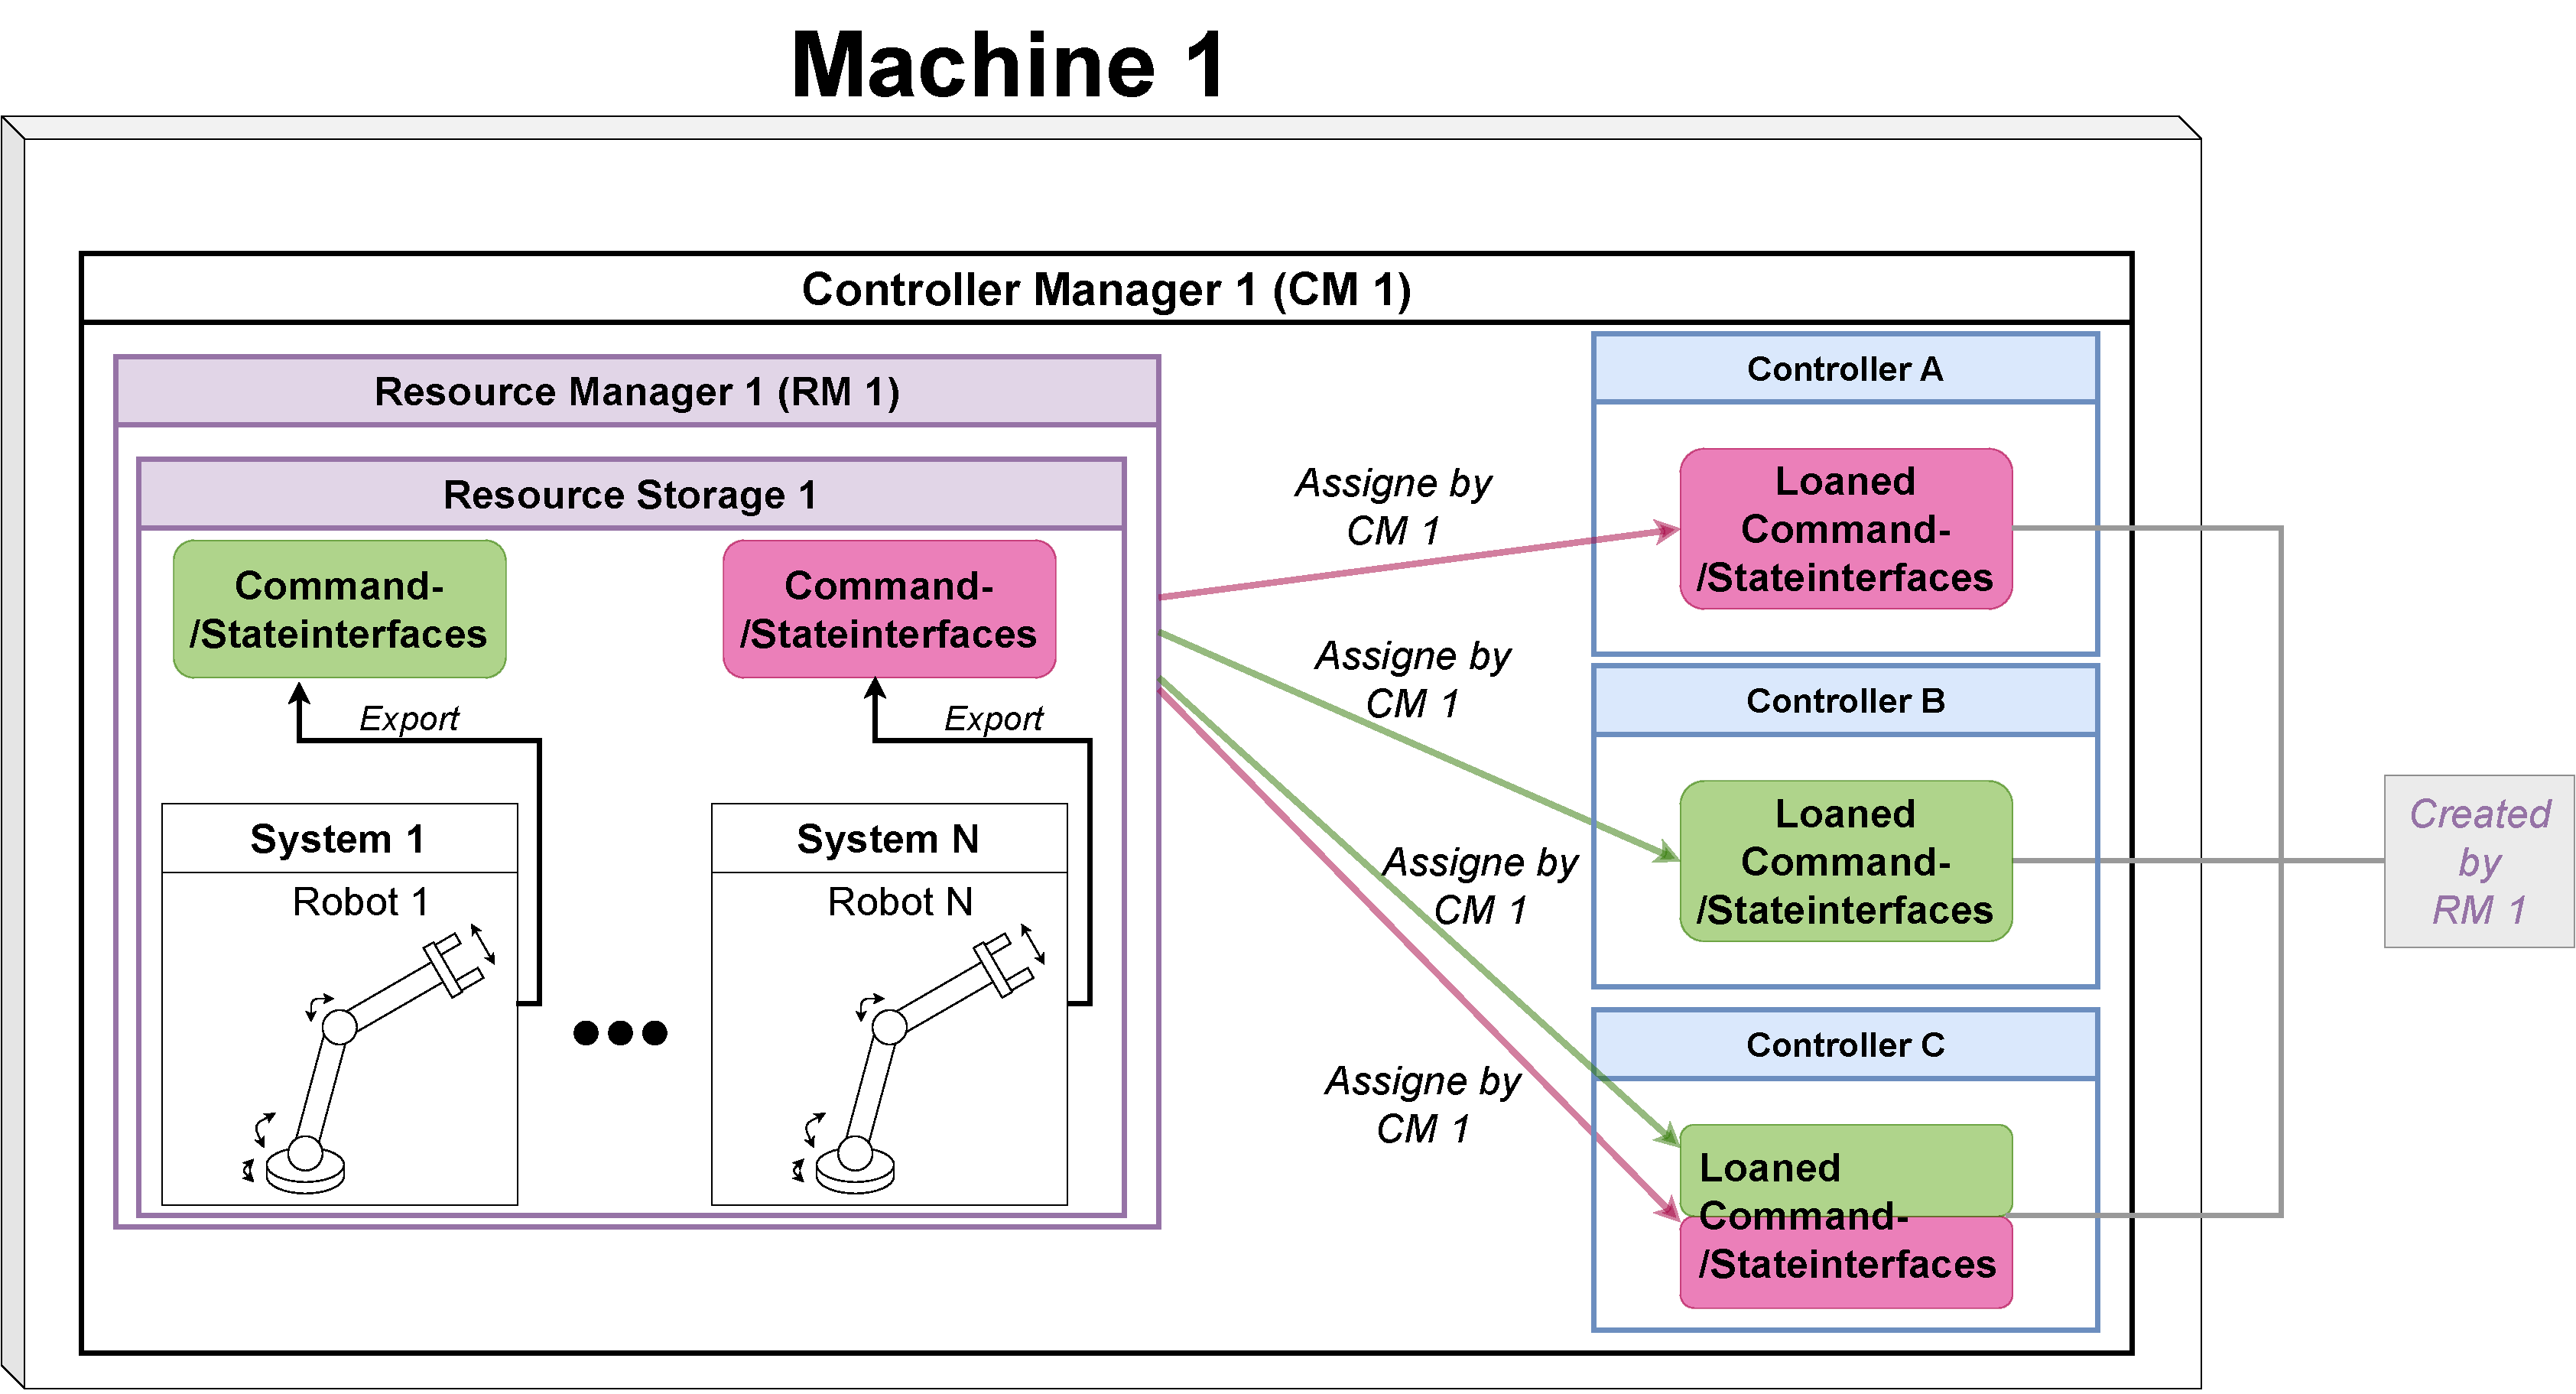
\includegraphics[width=1\textwidth]{Figures/c3/multiple_robots_one_system_current-Page-1.pdf}
	\caption{Schematic figure of how to realize a setup of multiple robots in \gls{r2c} where a tight synchronization between the robots is needed.}
	\label{c3_fig_r2c_mr_ts}
\end{figure}

\paragraph{Scenario 2:} 
In the second scenario, where no tight synchronization is needed and the robots act in a more or less independent manner, the most feasible way would be to have multiple machines with multiple controller managers running. Each controller manager would then have its own system. The system can then have its own controller architecture, which is managed by the corresponding controller manager. \newline
In this case, however, the systems are completely independent of each other. This means there is no synchronization between different systems possible. At least, there is no built-in functionality in \gls{r2c}. A schematic representation of this approach is provided in figure \ref{c3_fig_r2c_mr_is}.
\begin{figure}[H]
	\centering
	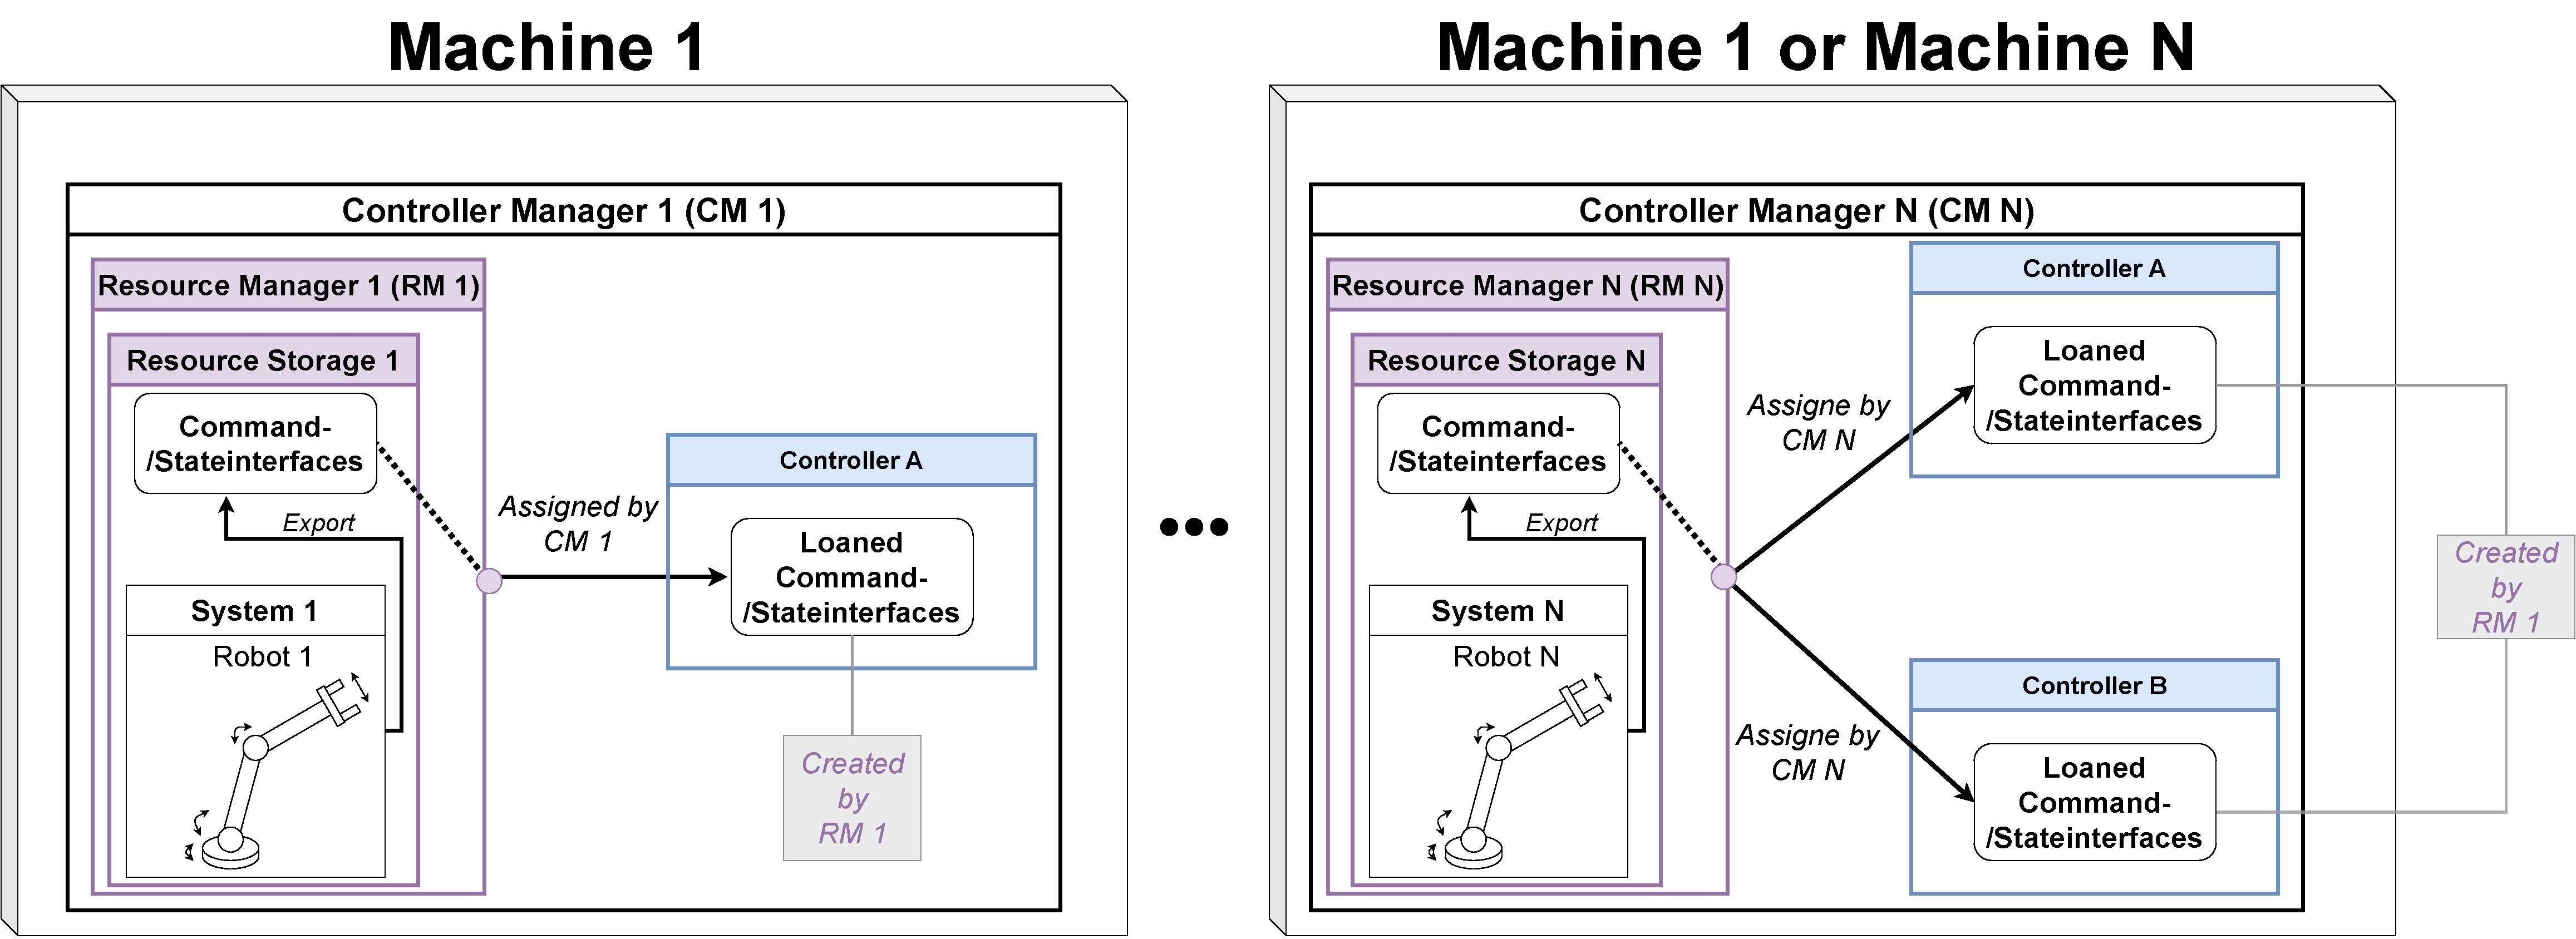
\includegraphics[width=1\textwidth]{Figures/c3/multiple_independent_robots_current.pdf}
	\caption{Schematic figure of how to realize a setup of multiple robots in \gls{r2c} where the robots act in an independent manner.}
	\label{c3_fig_r2c_mr_is}
\end{figure}





% \section{Time Synchronized Networks}
% What's the difference?????
% \section{Time Sensitive Networks}
